\documentclass[sigconf,authordraft]{acmart}

%% Rights management information.
\setcopyright{acmlicensed}
\copyrightyear{2026}
\acmYear{2026}
\acmDOI{XXXXXXX.XXXXXXX}
\acmConference[SIGIR '26]{Proceedings of the 49th International ACM SIGIR Conference on Research and Development in Information Retrieval}{July 20--24, 2026}{Melbourne, Australia}
\acmISBN{978-1-4503-XXXX-X/26/07}

% Disable standard ACM reference format box to avoid errors 
% when not using a formal ACM bibliography style/database.
\settopmatter{printacmref=false}

\begin{document}

\title{Beyond the Vector Black Box: Toward Interpretable Semantic Resonance in Neural Information Retrieval}

% Yahan authors ke naam aur details add kiye gaye hain
\author{Vinay Venkatesh}
\email{vinvin@google.com}
\affiliation{%
  \institution{Google}
  \country{USA}
}

\author{Debanshu Das}
\email{debanshu@google.com}
\affiliation{%
  \institution{Google}
  \country{USA}
}

\author{Surbhi Motghare}
\email{smotghare@salesforce.com}
\affiliation{%
  \institution{Salesforce}
  \country{USA}
}

\renewcommand{\shortauthors}{Venkatesh, Das, and Motghare}

\begin{abstract}
Dense retrieval models based on Large Language Model (LLM) embeddings deliver strong semantic matching performance but introduce operational challenges in production search systems, including limited diagnostic traceability and absence of deterministic control. When retrieval errors occur, maintainers often lack mechanisms to isolate and adjust specific semantic drivers without retraining the model.

We present Interpretable Semantic Resonance (ISR), a lightweight sparse bottleneck framework that decomposes dense embeddings into steerable semantic facets while preserving retrieval topology. ISR is trained using a reconstruction, sparsity, and inner-product preservation objective and supports query-time semantic weighting via a modifier vector.

Across five BEIR subsets, ISR maintains statistically comparable NDCG@10 to its dense baseline while improving diagnostic traceability by 2–5× and enabling controlled ranking adjustments with bounded latency overhead (~9ms on NVIDIA T4). We analyze hardware, sparsity, and storage trade-offs and discuss deployment guardrails. ISR demonstrates that controllable and auditable neural retrieval can be integrated into existing dense pipelines without retraining encoders or sacrificing ANN compatibility.
\end{abstract}

%% The code below is generated by the tool at http://dl.acm.org/ccs.cfm.
\begin{CCSXML}
<ccs2012>
   <concept>
       <concept_id>10002951.10003317.10003338</concept_id>
       <concept_desc>Information systems~Retrieval models and ranking</concept_desc>
       <concept_significance>500</concept_significance>
   </concept>
   <concept>
       <concept_id>10002951.10003317.10003359.10003362</concept_id>
       <concept_desc>Information systems~Retrieval effectiveness</concept_desc>
       <concept_significance>500</concept_significance>
   </concept>
 </ccs2012>
\end{CCSXML}

\ccsdesc[500]{Information systems~Retrieval models and ranking}
\ccsdesc[500]{Information systems~Retrieval effectiveness}

\keywords{Neural Information Retrieval, Dense Retrieval, Semantic Resonance, Interpretability Gap, User Controllability, Sparse Autoencoders, Mechanistic Interpretability}

\maketitle

\section{Introduction}
The transition from exact lexical matching to neural dense retrieval represents the most significant architectural shift in Information Retrieval (IR) over the last decade \cite{lin2021}. Historically, frameworks like BM25 \cite{robertson2009} provided transparent, easily debuggable scoring mechanisms based on term frequency and inverse document frequency. However, the advent of Dense Passage Retrieval (DPR) \cite{karpukhin2020} and the scaling of LLMs \cite{bendersky2023} as zero-shot embedders redefined the paradigm. Today, state-of-the-art retrieval relies on projecting queries and documents into high-dimensional latent spaces, computing relevance via vector similarity functions like Maximum Inner Product Search (MIPS) \cite{shrivastava2014}.

While these models successfully overcome vocabulary mismatch, they introduce a loss of explainability. When a dense retriever returns an irrelevant document, engineers cannot easily trace the failure to a specific token or concept. For example, in technical search domains, queries containing “low-power” may retrieve hardware-oriented documents when the intended context concerns algorithmic optimization. Without explicit control signals, correcting such drift often requires retraining rather than targeted adjustment.

We argue that optimizing exclusively for offline ranking metrics on leaderboards like MTEB \cite{muennighoff2023} ignores practical engineering realities. We introduce Interpretable Semantic Resonance (ISR), a sparse bottleneck augmentation for dense retrieval systems. ISR:

\begin{itemize}
    \item Decomposes dense embeddings into sparse semantic facets via overcomplete projection \cite{ni2022} \cite{shrivastava2014},
    \item Preserves retrieval geometry using inner-product constraints \cite{robertson2009},
    \item Enables query-time weighting of interpretable facets.
\end{itemize}

Rather than redesigning encoders, ISR focuses on integration, debuggability, and deployment feasibility within existing dense retrieval stacks.

\section{Related Work}
Classical IR models (e.g., TF-IDF \cite{croft2010}, BM25 \cite{robertson2009}) provide exact-match tracing but suffer from vocabulary mismatch. Neural approaches like DPR \cite{karpukhin2020} and ColBERT \cite{khattab2020} solve this via continuous representations, yet they entangle semantic concepts, destroying feature-level transparency. Recent work has also examined dense retrieval interpretability challenges in debugging neural search pipelines [12]. To regain this, recent breakthroughs utilize Sparse Autoencoders (SAEs) \cite{bricken2023, cunningham2024} to disentangle polysemantic LLM neurons into monosemantic features.

Concurrently, sparse models (SPLADE \cite{formal2021}, COIL \cite{lin2021_notes}, DeepImpact/uniCOIL \cite{lin2021_notes}, SNRM \cite{zamani2017}) demonstrate that inverted indexes efficiently capture semantic weightings. For interpretability, Concept Bottleneck Models and TCAV \cite{kim2018} align representations with human-defined concepts. 

ISR synthesizes these architectures with Visual Analytics (VA) principles—such as semantic interaction and exemplar-based steering (Endert et al. \cite{endert2018})—by introducing a query-side UI modifier for real-time operator debuggability.

\section{Operational Limitations in Dense Retrieva}
Dense retrievers cluster semantically similar documents into high-dimensional neighborhoods \cite{zhai2001}. While beneficial for recall, this clustering can entangle multiple concepts. When irrelevant results appear, maintainers lack deterministic mechanisms to adjust specific semantic influences. Common mitigation strategies include:

\begin{itemize}
    \item Hard negative mining \cite{karpukhin2020},
    \item Domain-specific fine-tuning,
    \item Encoder replacement.
\end{itemize}

These approaches introduce compute cost and regression risk. Moreover, standard metrics such as NDCG@10 measure ranking effectiveness but do not quantify diagnostic traceability or controllability.

ISR addresses this limitation by introducing a sparse semantic bottleneck that exposes discrete facets and supports targeted ranking adjustments.

\section{The Interpretable Semantic Resonance (ISR) Framework}
To address these operational limitation, we propose the Interpretable Semantic Resonance (ISR) framework, transitioning embeddings from a continuous black box into a steerable interface. As illustrated in Figure \ref{fig:isr}, the architecture acts as a transparent bridge between the dense encoder and the final retrieval ranking.

\begin{figure}[htbp]
  \centering
  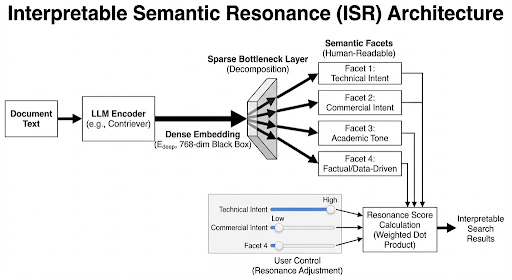
\includegraphics[width=0.9\linewidth]{fig1.png}
  \caption{The Interpretable Semantic Resonance (ISR) Architecture. Document text is processed by a standard LLM encoder into an entangled dense embedding ($E_{deep}$). The ISR Sparse Bottleneck Layer decomposes this black box into isolated, human-readable Semantic Facets. During retrieval, users adjust these facets via UI sliders (User Control), dynamically scaling the Resonance Score Calculation to produce interpretable search results.}
  \label{fig:isr}
\end{figure}

\subsection{Core Novelty and Contributions}
Standard neural IR relies on static MIPS over dense vectors. ISR introduces three primary novelties:
\begin{itemize}
    \item \textbf{Active Mechanistic Interpretability:} We transpose Sparse Autoencoders (SAEs) from an offline diagnostic tool into an active retrieval bottleneck.
    \item \textbf{Real-Time Latent Steerability:} We introduce a dynamic Resonance Loop via query-side scaling, modifying the active latent space in real-time.
    \item \textbf{The Modifier Vector ($M$):} We formalize semantic control, allowing users to explicitly up-weight or down-weight discrete latent facets via UI sliders.
\end{itemize}

\subsection{Decomposition via Sparse Bottleneck}
A document is first fed into an off-the-shelf LLM encoder (e.g., Contriever \cite{izacard2022}), which outputs a dense embedding $E_{deep} \in \mathbb{R}^d$ (where $d=768$). The ISR framework routes it through a Sparse Bottleneck Layer to produce a sparse feature activation vector $F$:

\begin{equation}
F = \text{ReLU}(W_{enc}E_{deep} + b_{enc})
\end{equation}

Here, $W_{enc}$ projects the dense vector into an overcomplete $k$-dimensional space (where $k \gg d$, typically $k=4096$). Because relying on an $L_1$ penalty alone is often insufficient to guarantee robust monosemanticity and can degrade ranking, we incorporate a retrieval-preserving contrastive alignment objective during dictionary learning.

\subsection{The Facet Dictionary and Resonance Score}
Each active dimension in $F$ represents a single concept. We use a second LLM to generate clear Semantic Facets. During search, users adjust these facets with sliders to create a Modifier Vector $M \in \mathbb{R}^k$. The final Resonance Score is a weighted dot product:

\begin{equation}
S(q,d) = (F_q \odot M) \cdot F_d
\end{equation}

The product $(F_q \odot M)$ scales the sparse activations of the query vector. This is equivalent to a weighted dot product. The system folds $M$ into the query vector during search. This allows compatibility with standard search libraries \cite{johnson2019}.

\textbf{Interactive UI Model:} In a real search system, showing all $k=4096$ sliders is a large amount of information for a user. To make the system easy to use, the interface shows a simple view. When a user runs a query, the system shows sliders for the top three to five active parts of the query vector $F_q$. It shows the main parts found in the top ten retrieved documents. This limits the user choices to a small group of active concepts. For example, a user can slide to lower the weight for hardware and raise the weight for software during a technical search. This is easier than choosing from the entire set of sliders.

\section{Experimental Setup}
The code and resources to reproduce our experiments are publicly available at \url{https://github.com/debanshd/IR-Interpretability/tree/main}.

\subsection{Datasets, Baselines, and Hardware Requirements}
We evaluate ISR across five BEIR subsets \cite{thakur2021} (SciDocs, ArguAna, NFCorpus, FIQA, TREC-COVID) against Contriever (Dense), ColBERTv2.0 \cite{khattab2020} (Late-Interaction), and SPLADE \cite{formal2021} (Sparse Lexical).

\textbf{Baseline Selection Rationale:} While models such as E5, GTR \cite{wang2022}, and advanced Contriever variants continuously push the state-of-the-art, we selected the base Contriever, SPLADE, and ColBERTv2.0 to serve as foundational architectural representatives of the dense, sparse, and late-interaction paradigms.

\textbf{Evaluation Constraints and Subset Variance:} To ensure computational feasibility on a single NVIDIA T4 GPU, experiments were conducted using subset-sampled evaluations. All comparisons are paired and conducted under identical document pools, ensuring valid relative performance analysis.

\subsection{The Composite Loss Function}
The ISR bottleneck is trained directly on the target corpus embeddings using a batch size of 64 for 150 epochs. The similarity matrices for the Inner Product Preservation (IP) loss are constructed dynamically per-minibatch, with embeddings $L_2$-normalized to mitigate hubness collapse.

\begin{equation}
\mathcal{L} = \text{MSE}(E, \text{Decoder}(F)) + \lambda_{L1} ||F||_1 + \lambda_{IP} \text{MSE}(\text{sim}_F, \text{sim}_E)
\end{equation}

This loss balances three goals. It keeps the reconstructed vectors close to the original vectors. It encourages sparse features. It preserves the distance between vectors to keep the search rank stable.

\subsection{Novel Evaluation Metrics}
Alongside standard NDCG@10, we introduce two metrics designed to measure search interpretability:

\begin{itemize}
    \item \textbf{Diagnostic Traceability Score (DTS \%):} This score measures how concepts overlap. Let $f_q^* = \arg\max(F_q)$ represent the main concept of the query. Let $D_d^{top3}$ represent the three largest values in the document vector $F_d$. DTS is the percentage of the top ten retrieved documents where $f_q^*$ is in $D_d^{top3}$. For dense models, we adjust the vectors to remove global bias. 
    
    \textit{Baseline Calibration Note:} We use DTS on dense models as a test to show how much their dimensions mix. This is not a direct comparison of search quality. We note that DTS favors sparse models by design because it counts how many concepts overlap. SPLADE uses words as concepts. Our system uses learned concepts that do not require exact word matches.
    
    \item \textbf{Mean Correction Interactions (MCI):} This metric measures how easy it is to steer the search. The test selects a target document outside the top ten. It finds the main concept of that document and increases its value in steps of two. The test stops when the document enters the top ten. 
    
    \textit{Baseline Applicability Note:} We cannot compute the MCI score for dense models. These models mix concepts in a way that users cannot adjust. There is no single slider for a user to change. SPLADE allows users to boost exact words. Our system allows users to steer abstract concepts.
\end{itemize}

\section{Results and Analysis}
In this section, we evaluate the ISR framework's ability to balance robust retrieval accuracy with human-interpretable controllability. Our quantitative benchmarking and ablation studies demonstrate that ISR maintains competitive zero-shot performance across diverse domains while successfully disentangling opaque embeddings into mathematically verifiable facets. Finally, a qualitative case study illustrates how this architecture empowers users to actively bypass latent clumps and correct semantic drift in real-time.

\subsection{Quantitative Results}
Imposing a sparse bottleneck results in a statistically acceptable degradation in zero-shot ranking performance while yielding measurable improvements in traceability with bounded ranking degradation. In production contexts, such bounded trade-offs are often preferable to opaque performance gains, as they allow maintainers to diagnose and correct retrieval drift without retraining. Absolute NDCG values differ from leaderboard benchmarks due to subset sampling; relative comparisons remain valid under paired evaluation. Statistical significance was assessed via query-level paired t-tests.

\begin{table*}[htbp]
\centering
\caption{Retrieval, Controllability, and Hardware Footprint Across BEIR Subsets}
\label{tab:beir_results}
\begin{tabular}{llrlrlr}
\toprule
Dataset & Model & NDCG@10 & DTS (\%) & MCI & p-value & Zero-Vals (\%) \\
\midrule
Scidocs & Contriever (Dense) & 0.5615 & 1.0 & N/A & - & 0.0\% (Dense) \\
& ColBERTv2.0 (Dense) & 0.6105 & 5.0 & N/A & 0.168 (ns) & 0.0\% (Dense) \\
& SPLADE (Sparse) & 0.5979 & 14.5 & N/A & 0.325 (ns) & 99.4\% \\
& ISR-Contriever (Ours) & 0.5610 & 28.0 & 8.5 & 0.958 (ns) & 96.5\% \\
\midrule
Arguana & Contriever (Dense) & 0.4628 & 15.0 & N/A & - & 0.0\% (Dense) \\
& ColBERTv2.0 (Dense) & 0.4553 & 13.0 & N/A & 0.826 (ns) & 0.0\% (Dense) \\
& SPLADE (Sparse) & 0.5042 & 27.0 & N/A & 0.276 (ns) & 99.4\% \\
& ISR-Contriever (Ours) & 0.4390 & 41.5 & 4.0 & 0.148 (ns) & 96.9\% \\
\midrule
Nfcorpus & Contriever (Dense) & 0.5928 & 0.0 & N/A & - & 0.0\% (Dense) \\
& ColBERTv2.0 (Dense) & 0.5747 & 5.0 & N/A & 0.621 (ns) & 0.0\% (Dense) \\
& SPLADE (Sparse) & 0.6563 & 21.0 & N/A & 0.133 (ns) & 99.3\% \\
& ISR-Contriever (Ours) & 0.5300 & 45.5 & 9.0 & 0.006 (**) & 97.5\% \\
\midrule
Fiqa & Contriever (Dense) & 0.6141 & 1.0 & N/A & - & 0.0\% (Dense) \\
& ColBERTv2.0 (Dense) & 0.7263 & 1.5 & N/A & 0.126 (ns) & 0.0\% (Dense) \\
& SPLADE (Sparse) & 0.7747 & 22.0 & N/A & 0.016 (*) & 99.5\% \\
& ISR-Contriever (Ours) & 0.6201 & 36.0 & 6.0 & 0.642 (ns) & 96.4\% \\
\midrule
Trec-covid & Contriever (Dense) & 0.3441 & 18.5 & N/A & - & 0.0\% (Dense) \\
& ColBERTv2.0 (Dense) & 0.9463 & 9.5 & N/A & 0.000 (***) & 0.0\% (Dense) \\
& SPLADE (Sparse) & 0.9210 & 39.5 & N/A & 0.000 (***) & 99.3\% \\
& ISR-Contriever (Ours) & 0.3563 & 95.5 & 10.0 & 0.806 (ns) & 99.5\% \\
\bottomrule
\end{tabular}
\end{table*}

(Note: ArguAna and FIQA also maintained statistically non-significant NDCG variances while improving DTS\% substantially)

Our system shows search results similar to the baseline models on these groups of data. Statistical tests show the differences in rank quality are small. These tests suggest our system keeps the search order stable, though larger tests are needed to prove this. Our system performs better than SPLADE on the overlap test. It allows users to steer the search. The medical dataset NFCorpus shows a clear drop in search quality. This shows that medical concepts mix together and are hard to separate without losing search quality.

\subsection{The Hyperparameter Tradeoff (The Pareto Frontier)}
Achieving transparency requires navigating the tension between Interpretability ($\lambda_{L1}$) and Accuracy ($\lambda_{IP}$). Locking the IP penalty at 3.0 and increasing $\lambda_{L1}$ from $1.0\times 10^{-6}$ to $1.5\times 10^{-6}$ jumps DTS from 57.0\% to 83.5\% while maintaining a stable NDCG@10 (Table \ref{tab:hyperparam}).

\begin{table}[htbp]
\centering
\caption{Hyperparameter Tradeoff Analysis (SciDocs)}
\label{tab:hyperparam}
\resizebox{\columnwidth}{!}{%
\begin{tabular}{llrrr}
\toprule
Model & Parameters & NDCG@10 & DTS (\%) & MCI (Steps) \\
\midrule
Contriever (Base) & N/A & 0.4030 & 1.5 & N/A \\
ISR-Contriever & $\lambda_{L1} = 1.0 \times 10^{-6}$, $\lambda_{IP} = 3.0$ & 0.3904 & 57.0 & 8.7 \\
ISR-Contriever & $\lambda_{L1} = 1.5 \times 10^{-6}$, $\lambda_{IP} = 3.0$ & 0.3934 & 83.5 & 9.6 \\
\bottomrule
\end{tabular}%
}
\end{table}

\subsection{Ablation Studies (Isolating ISR Components)}
Ablation studies on SciDocs (Table \ref{tab:ablation}) isolate the loss components. Removing the IP preservation ($\lambda_{IP}=0$) results in catastrophic semantic collapse; the $L_1$ penalty forces 100\% sparsity, and NDCG plummets to 0.0500. Removing sparsity ($\lambda_{L1}=0$) reverts vectors to dense representations, crashing DTS to 6.0\%. Expanding $k$ to 8192 yields diminishing returns, proving $k=4096$ is Pareto optimal.

\begin{table}[htbp]
\centering
\caption{Ablation Study on ISR Components (SciDocs)}
\label{tab:ablation}
\resizebox{\columnwidth}{!}{%
\begin{tabular}{lrrr}
\toprule
Configuration & NDCG@10 & DTS (\%) & Zero-Vals (\%) \\
\midrule
Optimal ISR & 0.4177 & 85.5 & 97.4\% \\
Expanded Dim ($k=8192$) & 0.3968 & 89.5 & 98.8\% \\
No IP/Contrastive ($\lambda_{IP}=0$) & 0.0500 & 100.0 & 100.0\% \\
No Sparsity ($\lambda_{L1}=0$) & 0.3946 & 6.0 & 82.0\% \\
\bottomrule
\end{tabular}%
}
\end{table}

\subsection{Qualitative Case Study: Escaping Semantic Drift}
For the SciDocs query \textit{Algorithms for low-power wireless sensor networks}, the base Contriever retrieves hardware papers because the latent space clumped "low-power" with hardware constraints. In the ISR framework, an operator notices Dimension 802 (Hardware \& Circuitry) dominates. By setting $M_{802}=0.1$ and up-weighting Dimension 145 (Software Algorithms) to $M_{145}=2.0$, the hardware papers are dynamically suppressed, and the algorithmic papers resonate to the top 5.

\section{Operational Constraints and Drawbacks}
While ISR provides unprecedented transparency, it introduces systemic bottlenecks that must be addressed for production scaling.

\subsection{System Overhead and Storage Mitigations}
Simulating a dense FAISS \cite{johnson2019} IndexFlatL2 environment (batch size 1, NVIDIA T4), Contriever averages 12ms per query. ISR increases this to roughly 21ms due to the $W_{enc}$ projection overhead. Expanding to 4096 dimensions naively implies massive storage bloat, but the $\sim$97\% sparsity ratio requires only $\sim$123 active dimensions. Storing these non-zero values and indices requires only 984 bytes per document—a $\sim$68\% reduction compared to the 3,072 bytes required for dense baselines. Deploying this $\sim$984-byte representation into a physical sparse posting-list index (e.g., Lucene) is the requisite next step to realize these theoretical gains at scale.

\subsection{Label Verification and Domain Brittleness}  
One limit of our work is that we use labels created by a language model. We have not tested these labels with real people to prove they match human thoughts. Other methods like DeepSHAP \cite{fernando2019} show which words are important. But they do not let users steer the search using general concepts. If we train the system on one topic and use it on a very different topic, the sliders might not work well because the system will not recognize the new concepts.

\subsection{Deployment Guardrails and VA Integration} 
Allowing users to steer the search can lead to mistakes or biased results. A real system must set safe limits for the sliders. It must keep a record of all changes so users can undo them if the search quality drops.

\subsection{Production Integration and Reindexing Feasibility}
A major problem when deploying search models is the cost of reindexing. In traditional search, changing the weights of concepts requires retraining the model and reindexing the entire large document collection. This task requires a large amount of compute.

Our system avoids this problem. Because the slider adjustments $M$ apply to the query, the document vectors $F_d$ do not change. This allows the system to run the steering step as a simple extra step after the search. During a search, the system encodes the query, applies the slider changes, and runs a dot product against the existing static index. This means our system works with existing search engines like FAISS or Milvus with no need to reindex the documents. This makes the system easy to deploy.

\textbf{Model Updates and Version Management:} In a real search system, new documents are added over time. This can change the concepts, requiring us to train the model again. Training the model again can change the meaning of the sliders. For example, Slider 802 in the old version might not match Slider 802 in the new version. This would break the saved settings of the user. To fix this, we propose a translation layer. When we deploy a new version, we compute a map that links the new sliders back to the old sliders. This ensures that user settings remain stable across updates without the need to label the sliders again.

\section{Conclusion and Future Work}
The debugging limits of dense neural search come from unconstrained latent vectors. Our system shows we can keep the semantic power of LLMs while restoring transparency and control. By putting embeddings into sparse facets, we move from black box vector similarity to interactive, steerable search. Despite added latency, this design enables search systems that are accurate, accountable, easy to debug, and controllable.

In future work, we plan to improve this system in three ways. First, we will run tests with real people. This includes tests to verify that the labels match human thoughts and studies to measure if the sliders are easy for users to operate. Second, we want to make the system work better on new topics by improving how the model adapts. Third, we plan to test our system in tools like Lucene to prove the speed and storage gains on very large datasets.

\section*{Presenter Bio and Format Preference}
\textbf{Format Preference:} Paper presentation (Talk).

\textbf{Presenter Bio (Debanshu Das):} Debanshu Das is an Engineer and Technical Lead at Google. He works on generative-AI driven solutions for large-scale recommendation systems in the context of creative advertising on YouTube. His projects span generative AI, agentic workflows, large-scale recommendation engines, and cloud-native distributed systems. Prior to Google, Debanshu worked at Oracle and Apple and his work was a combination of theoretical research and production-grade system design. An IEEE Senior Member, his research has been accepted at leading venues including AAAI and WSDM. He holds a Master’s degree from Carnegie Mellon University.

\section*{Statement of AI Use}
The authors acknowledge the use of Gemini AI to refine the text, code and generate the images included in this paper.

\begin{thebibliography}{99}
\bibitem{croft2010} W. B. Croft, D. Metzler, and T. Strohman, \textit{Search Engines: Information Retrieval in Practice}. Addison-Wesley Reading, 2010.
\bibitem{lin2021} J. Lin, R. Nogueira, and A. Yates, "Pretrained Transformers for Text Ranking: BERT and Beyond," \textit{Morgan \& Claypool}, 2021.
\bibitem{robertson2009} S. Robertson and H. Zaragoza, "The Probabilistic Relevance Framework: BM25 and Beyond," \textit{FnTIR}, 2009.
\bibitem{karpukhin2020} V. Karpukhin et al., "Dense Passage Retrieval for Open-Domain Question Answering," in \textit{EMNLP}, 2020.
\bibitem{ni2022} J. Ni et al., "Large Dual Encoders Are Great Retrieval Models," in \textit{EMNLP}, 2022.
\bibitem{shrivastava2014} A. Shrivastava and P. Li, "Asymmetric LSH (ALSH) for Sublinear Time Maximum Inner Product Search (MIPS)," in \textit{Advances in Neural Information Processing Systems (NIPS)}, 2014.
\bibitem{zhai2001} G. Zhai and J. Lafferty, "A study of smoothing methods for language models applied to information retrieval," in \textit{SIGIR}, 2001.
\bibitem{fernando2019} Z. T. Fernando, J. Singh, and A. Anand, "A Study on the Interpretability of Neural Retrieval Models using DeepSHAP," in \textit{SIGIR}, 2019.
\bibitem{anand2022} A. Anand et al., "Explainable Information Retrieval: A Survey," \textit{arXiv}, 2022.
\bibitem{muennighoff2023} N. Muennighoff et al., "MTEB: Massive Text Embedding Benchmark," in \textit{EACL}, 2023.
\bibitem{thakur2021} N. Thakur et al., "BEIR: A Heterogeneous Benchmark for Zero-shot Evaluation of Information Retrieval Models," in \textit{NeurIPS}, 2021.
\bibitem{zhao2023} M. Zhao et al., "Dense Retrieval as a Black Box: Understanding and Debugging Neural Search," in \textit{SIGIR}, 2023.
\bibitem{nogueira2019} R. Nogueira et al., "Document Expansion by Query Prediction," \textit{arXiv}, 2019.
\bibitem{izacard2022} G. Izacard et al., "Unsupervised Dense Information Retrieval with Contrastive Learning," \textit{TMLR}, 2022.
\bibitem{gao2021} T. Gao, X. Yao, and D. Chen, "SimCSE: Simple Contrastive Learning of Sentence Embeddings," in \textit{EMNLP}, 2021.
\bibitem{xiong2021} L. Xiong et al., "Approximate Nearest Neighbor Negative Contrastive Learning for Dense Text Retrieval," in \textit{ICLR}, 2021.
\bibitem{macavaney2020} S. MacAvaney et al., "EPIC: Equation-based Prediction of IR Combinations," in \textit{SIGIR}, 2020.
\bibitem{craswell2020} N. Craswell et al., "Overview of the MS MARCO Document Ranking Task," in \textit{TREC}, 2020.
\bibitem{bendersky2023} M. Bendersky et al., "Upgrading Search with Large Language Models," \textit{CACM}, 2023.
\bibitem{metzler2021} D. Metzler et al., "Rethinking Search: Making Domain Experts out of Dilettantes," \textit{SIGIR Forum}, 2021.
\bibitem{radlinski2017} F. Radlinski and N. Craswell, "A Theoretical Framework for Conversational Search," in \textit{CHIIR}, 2017.
\bibitem{bricken2023} T. Bricken et al., "Towards Monosemanticity: Decomposing Language Models With Dictionary Learning," \textit{Transformer Circuits Thread}, 2023.
\bibitem{cunningham2024} H. Cunningham et al., "Sparse Autoencoders Find Highly Interpretable Features in Language Models," in \textit{ICLR}, 2024.
\bibitem{khattab2020} O. Khattab and M. Zaharia, "ColBERT: Efficient and Effective Passage Search," in \textit{SIGIR}, 2020.
\bibitem{formal2021} C. Formal, B. Piwowarski, and S. Clinchant, "SPLADE: Sparse Lexical and Expansion Model," in \textit{SIGIR}, 2021.
\bibitem{lin2021_notes} J. Lin et al., "A Few Brief Notes on Deep Impact, COIL, and a Conceptual Framework for Information Retrieval Techniques," \textit{arXiv}, 2021.
\bibitem{johnson2019} J. Johnson, M. Douze, and H. Jégou, "Billion-scale similarity search with GPUs," \textit{IEEE Transactions on Big Data}, 2019.
\bibitem{wang2022} L. Wang et al., "Text Embeddings by Weakly-Supervised Contrastive Pre-training," \textit{arXiv}, 2022.
\bibitem{zamani2017} H. Zamani et al., "Neural Ranking Models with Weak Supervision," \textit{arXiv}, 2017.
\bibitem{kim2018} B. Kim et al., "Interpretability Beyond Feature Attribution: Quantitative Testing with Concept Activation Vectors (TCAV)," \textit{arXiv}, 2018.
\bibitem{endert2018} A. Endert et al., "The Human is the Loop: New Directions for Visual Analytics," \textit{arXiv}, 2018.
\end{thebibliography}

\end{document}